\documentclass{article}
\usepackage[utf8]{inputenc}
\usepackage{graphicx}

\title{Antworten zu Aufgabenblatt 1}
\date{2019-06-04}
\author{Alexander Lüngen}

\begin{document}
    \maketitle
    \newpage
    \section{Aufgabe 1}
        \subsection{a)}
        Die Reihenfolge in welcher die IDs der Threads ausgegeben werden ist nicht immer gleich.
        \subsection{b)}
	\begin{tabular}{|l|l|r|r|r|}
		\hline
		- & Number of Threads & N & Time & Speedup \\
		\hline
		manual & 2 & 10 & 0:00 & 0.8 \\
		 & 2 & 100 & 0:00 & 0.8 \\
		 & 2 & 1000 & 0:00 & 0.8 \\
		 & 2 & 10000 & 0:00 & 0.8 \\
		 & 4 & 10 & 0:00 & 0.8 \\
		 & 4 & 100 & 0:00 & 0.8 \\
		 & 4 & 1000 & 0:00 & 0.8 \\
		 & 4 & 10000 & 0:00 & 0.8 \\
		 & 8 & 10 & 0:00 & 0.8 \\
		 & 8 & 100 & 0:00 & 0.8 \\
		 & 8 & 1000 & 0:00 & 0.8 \\
		 & 8 & 10000 & 0:00 & 0.8 \\
		 & 16 & 10 & 0:00 & 0.8 \\
		 & 16 & 100 & 0:00 & 0.8 \\
		 & 16 & 1000 & 0:00 & 0.8 \\
		 & 16 & 10000 & 0:00 & 0.8 \\
		 & 32 & 10 & 0:00 & 0.8 \\
		 & 32 & 100 & 0:00 & 0.8 \\
		 & 32 & 1000 & 0:00 & 0.8 \\
		 & 32 & 10000 & 0:00 & 0.8 \\
		\hline
		reductino & 2 & 10 & 0:00 & 0.8 \\
		 & 2 & 100 & 0:00 & 0.8 \\
		 & 2 & 1000 & 0:00 & 0.8 \\
		 & 2 & 10000 & 0:00 & 0.8 \\
		 & 4 & 10 & 0:00 & 0.8 \\
		 & 4 & 100 & 0:00 & 0.8 \\
		 & 4 & 1000 & 0:00 & 0.8 \\
		 & 4 & 10000 & 0:00 & 0.8 \\
		 & 8 & 10 & 0:00 & 0.8 \\
		 & 8 & 100 & 0:00 & 0.8 \\
		 & 8 & 1000 & 0:00 & 0.8 \\
		 & 8 & 10000 & 0:00 & 0.8 \\
		 & 16 & 10 & 0:00 & 0.8 \\
		 & 16 & 100 & 0:00 & 0.8 \\
		 & 16 & 1000 & 0:00 & 0.8 \\
		 & 16 & 10000 & 0:00 & 0.8 \\
		 & 32 & 10 & 0:00 & 0.8 \\
		 & 32 & 100 & 0:00 & 0.8 \\
		 & 32 & 1000 & 0:00 & 0.8 \\
		 & 32 & 10000 & 0:00 & 0.8 \\
		\hline
	\end{tabular}
        \subsection{c)}
	\begin{center}
		
\includegraphics[width=0.6\linewidth]{Aufgaben-Ressourcen/normal-1000.jpg}	
	\end{center}

	\begin{center}
		
\includegraphics[width=0.4\linewidth]{Aufgaben-Ressourcen/critical-1000.jpg}\quad
\includegraphics[width=0.4\linewidth]{Aufgaben-Ressourcen/critical-1000-1000.jpg}
		\\[\baselineskip]
		\includegraphics[width=0.4\linewidth]{Aufgaben-Ressourcen/critical-10000-1000.jpg}\quad\includegraphics[width=0.4\linewidth]{Aufgaben-Ressourcen/critical-10000-1000.jpg}
	\end{center}


    \section{Aufgabe 2}
    	\subsection{a)}
		\begin{enumerate}
			\item Example: Es besteht eine Race-Condition auf dem Array a über Index i,
				bei ungünstiger Ausführungsreihenfolge der Threads kann es dazu kommen,
				das a[i] durch einen Thread geschrieben wird und von einem anderen Thread versucht wird, darauf in der nachfolgenden Anweisung lesend zuzugreifen.
				Um dieses Problem zu lösen können zwei for-Schleifen verwendet werden.
				Eine schreibt alle Werte in Array a und die zweite schreibt alle Werte unter Zugriff auf Array a in Array b. 
				Beide Schleifen werden jeweils getrennt parallelisiert.
			\item Example: Threads exisiteren hier in der gesamten parallelen Region.
				Das nowait-Statement der ersten parallelisierten For-Schleife bewirkt, dass Threads bereits die nächste parallelisierte Schleife bearbeiten können, wenn sie ihren Teil der ersten Schleife fertig verarbeitet haben.
				Dies führt zu einer Race-Condition auf das Array a mit Index i, ähnlich zu Example 1.
				Mit dem entfernen des nowait-Statements der ersten for-Schleife warten alle Threads wieder auf die implizite Barriere bis alle Threads fertig sind und es kann Problemlos auf die geschriebenen Werte in Array a zugegriffen werden.
			\item Example: Hier ist die Variable x zunächst global definiert und wird somit implizit zwischen den Threads geshared. 
				Somit besteht eine Race-Condition auf x da die Threads unabhängig voneinander sowohl lesend als auch schreibend auf x zugreifen.
				Indem man x explizit als private deklariert, erhält jeder Thread seine eigene Kopie der Variable und es besteht keine Race-Condition mehr.
			\item Example: f ist global definiert und wird durch jeden Thread private gesetzt. 
				Allerdings erhält jeder Thread eine uninitialiserte Kopie der Variable f, was bedeutet das dass initialisieren mit dem Wert 2 vor der Schleife nur für den Master-Thread sichtbar ist.
				Um diese Initialiserung auch für alle übrigen Threads sichtbar zu machen, ist es erforderlich, f mittels firstprivate zu deklarieren.
				Des weiteren wird der Wert von x nicht aus der parallelen Region wieder rausgeschrieben, sondern gelöscht. 
				Wodurch der zuletzt geschriebene Wert innerhalb der parallelen Region in x nach außen hin nicht sichtbar ist.
				Um deses Verhalten zu erreichen, muss x als lastprivate deklariert werden.
			\item Example:

		\end{enumerate}

	\subsection{b)}

    \section{Aufgabe 3}
        \subsection{a)}
        Speedup:
        Effizienz:
        \subsection{b)}
        Race-Conditions: Wenn zwei Threads unabhängig voneinander auf eine Ressource lesend oder auch schreibend zugreiffen können, 
        spricht man von einer Race-Condition. Hierbei kann es bspw. beim Zugriff auf Variablen bei ungünstiger Ausführungszeiten
        dazu kommen, dass am Ende der Berechnungen ein falscher Wert in der Variable enthalten ist, als wenn die Berechnung sequentiell 
        ausgeführt worden wäre.
        Um eine Race-Condition zu vermeiden, können die kritischen Abschnitte in der Art und weise gesichert werden, das immer nur ein 
        Thread gleichzeitig innerhalb des kritischen Abschnitts sein darf.

        In diesem Zusammenhang kann es auch zu Deadlocks, Lifelocks oder auch Starvation kommen. 
        \subsection{c)}
        CPU
        GPGPU
        FPGA
        MICs

    \section{Aufgabe 4}

    \section{Aufgabe 5}
	\subsection{a)}
	f(x,y) muss definiert sein auf $\Omega$ \newline
	$\Gamma$ ist der Rand von $\Omega$  \newline
	L\"{o}sung u(x,y) muss zweifach differenzierbar sein 
	\subsection{b)}
	f(x,y) = ($N^2$ + $M^2$)*4*$\pi^2$*sin(2*M*$\pi$*x)*sin(2*N*$\pi$*y)
	\subsection{c)}
	Es handelt sich um eine h-FEM.  \newline
	Folgende Lösungswerte ergaben sich mit M=3; N=2; l=5,6,7;  \newline
\begin{figure}
	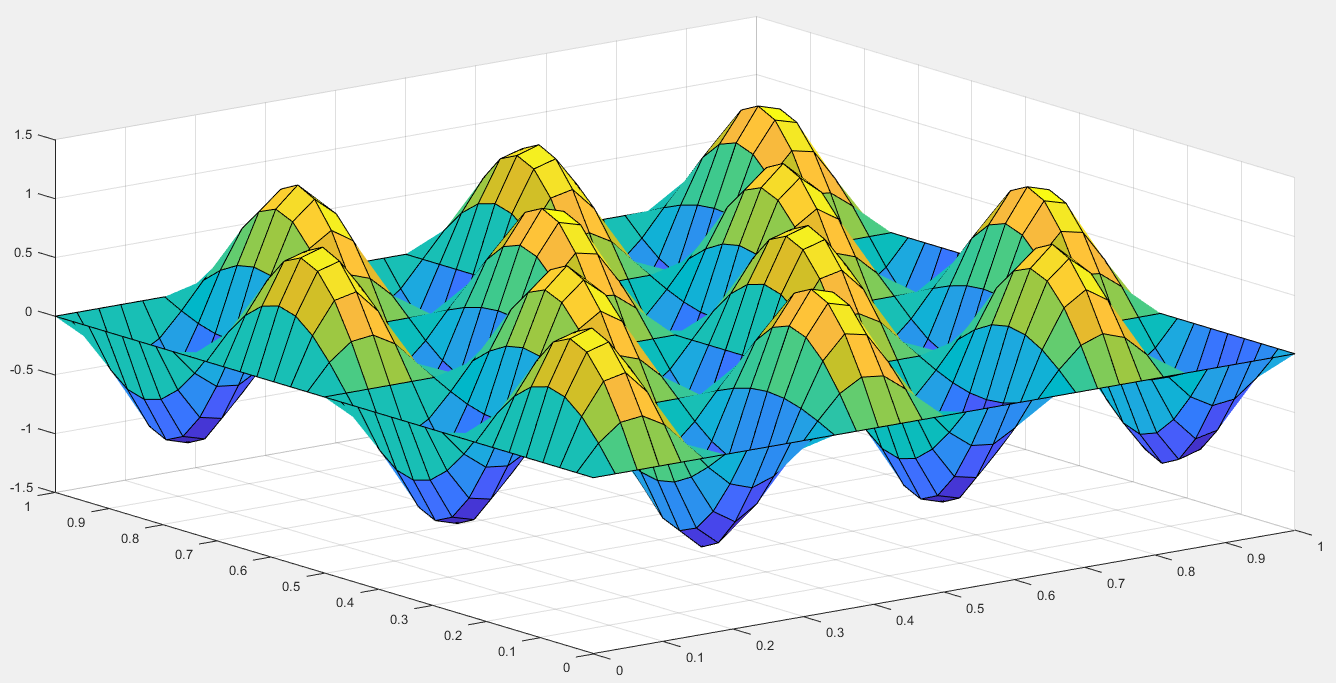
\includegraphics[width=0.8\linewidth]{Aufgaben-Ressourcen/A5L5M3N2.png} 
		\caption{l=5; h=1/32;}
\end{figure}
\begin{figure}
	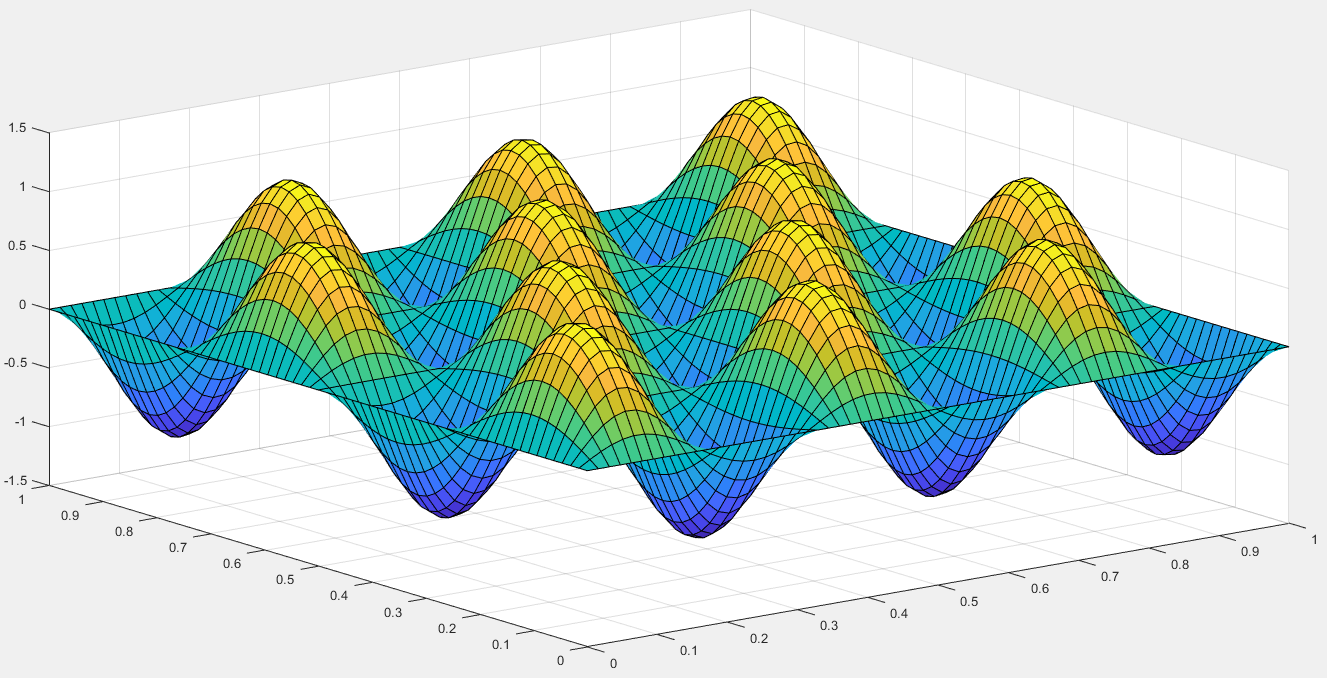
\includegraphics[width=0.8\linewidth]{Aufgaben-Ressourcen/A5L6M3N2.png} 
		\caption{l=6; h=1/64;}
\end{figure}
\begin{figure}
	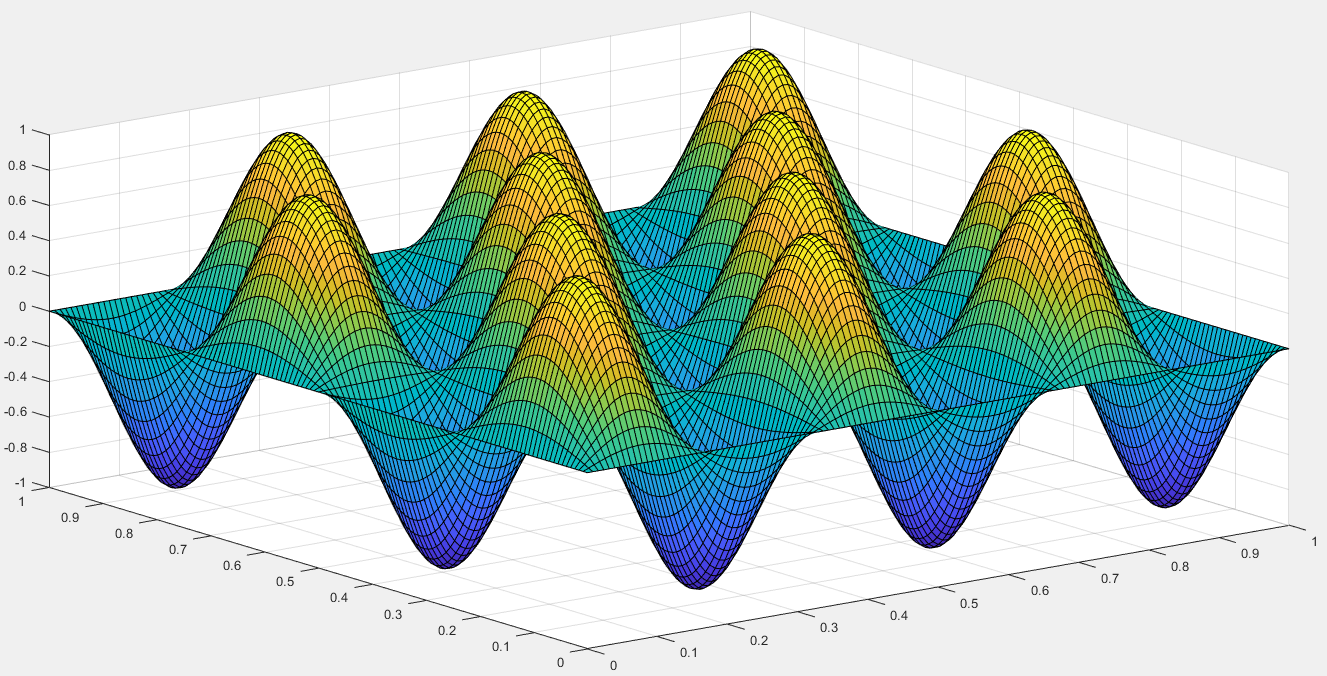
\includegraphics[width=0.8\linewidth]{Aufgaben-Ressourcen/A5L7M3N2.png}
		\caption{l=7; h=1/128;}
\end{figure}

\section{Aufgabe 6}
	\subsection{a)}
	\subsection{b)}
	\subsection{c)}
	\subsection{d)}
\section{Aufgabe 7}
\end{document}
